%          spconf.sty  - ICASSP/ICIP LaTeX style file, and
%          IEEEbib.bst - IEEE bibliography style file.
% --------------------------------------------------------------------------
\documentclass{article}
\usepackage{spconf,amsmath,graphicx}
\usepackage{booktabs}
\usepackage{hyperref}
\usepackage{caption}

% Title.
% ------
\title{Resilient Security: Threat Modeling and Defensive Strategies for Large Language Models Platforms}
\name{SN: 24076607}
\address{}
%
\begin{document}

\maketitle
%
\begin{abstract}
    This report presents a comprehensive approach to securing Large Language Model (LLM) platforms through threat modeling and defensive strategy development. We analyze a Flask-based AI dialogue system with user authentication, conversation management, and content moderation capabilities. 
    Using STRIDE methodology, we identify and prioritize threats including session hijacking, brute force attacks, NoSQL injection, and DDoS attempts, demonstrating through practical simulations how adversaries could extract sensitive information. 
    We then implement a multi-layered defense incorporating MFA, bcrypt password hashing, rate limiting, HTTPS encryption, and AI-driven content filtering to prevent storing prohibited content. 
    The paper addresses regulatory compliance with GDPR, CRA, and PSTI frameworks while considering ethical implications of AI security systems. 
    Finally, we evaluate enterprise scaling considerations and innovative approaches like contextual authentication and privacy-preserving techniques to ensure long-term viability of secure LLM platforms.\footnote{The code is provided on GitHub: \url{https://github.com/yushiran/ELEC0138Coursework\_Group5}, and the presentation video is available at: \url{https://www.youtube.com/watch?v=0v1x2g4X8nE}.}
\end{abstract}
%
\begin{keywords}
    Large Language Models, threat modeling, cybersecurity, authentication, privacy, STRIDE, defensive strategies, ethical AI
\end{keywords}

\section{Coursework 1: Threat Modeling \& Attack Simulation}
\subsection{Introduction and objectives}
This project simulates a widely used AI dialogue model system developed using Flask (Python) and MongoDB, creating a user login, a registration interface and a LLM chat interface. The system stores the user account password and other related personal information in the MongoDB database, and the user's chat information is also stored in the associated database to protect and manage it. 
At the same time, machine learning is used to load the LLM to identify and delete banned messages in the chat to prevent the database from being contaminated with banned messages.
The system will include the following elements, which will be analysed:
\begin{enumerate}
    \item Front-end HTML forms: login, registration, AI chat interface, etc.
    \item Back-end: a Flask-based server that manages user information and dialogue content.
    \item Database: MongoDB (local instance) to store user data and messages.
\end{enumerate}

First, when the webpage is opened, the interface is shown in the diagram below. Fig. \ref{fig:login} shows the system login interface and Fig. \ref{fig:registration} shows the registration interface that the system retrieves.
\begin{figure}[htb]
    \centering
    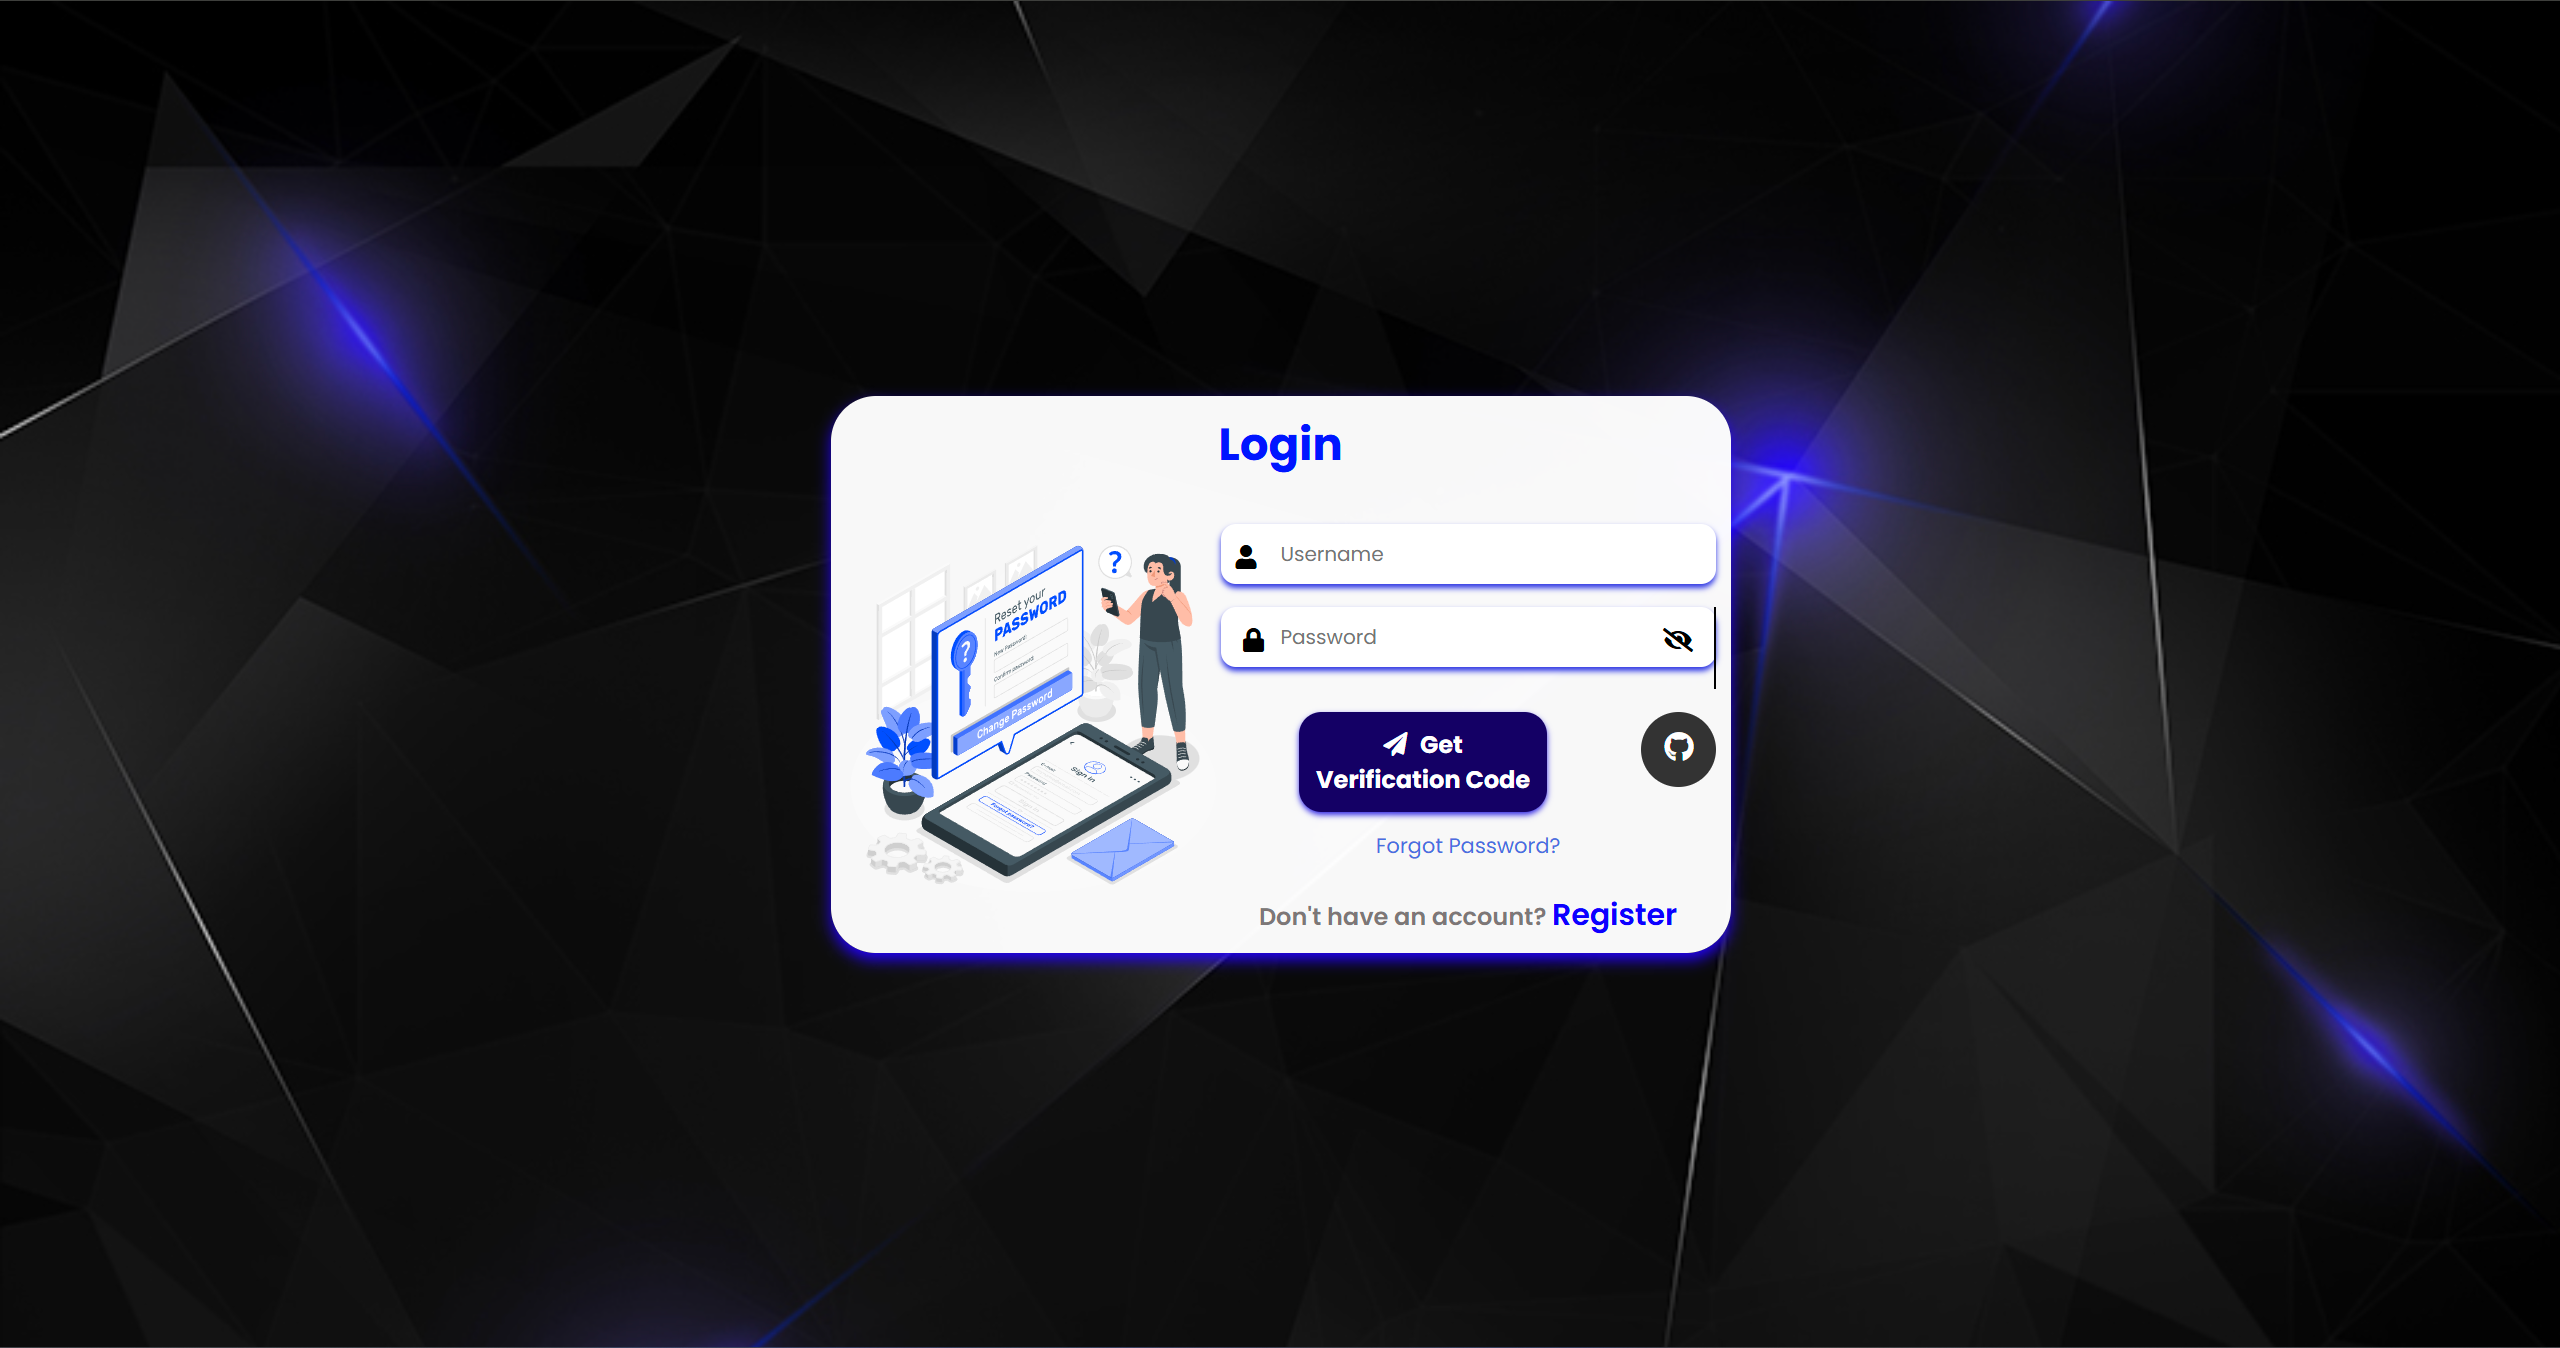
\includegraphics[width=0.5\textwidth]{images/login_screenshot.png}
    \caption{Login interface of the system}
    \label{fig:login}
\end{figure}

\begin{figure}[htb]
    \centering
    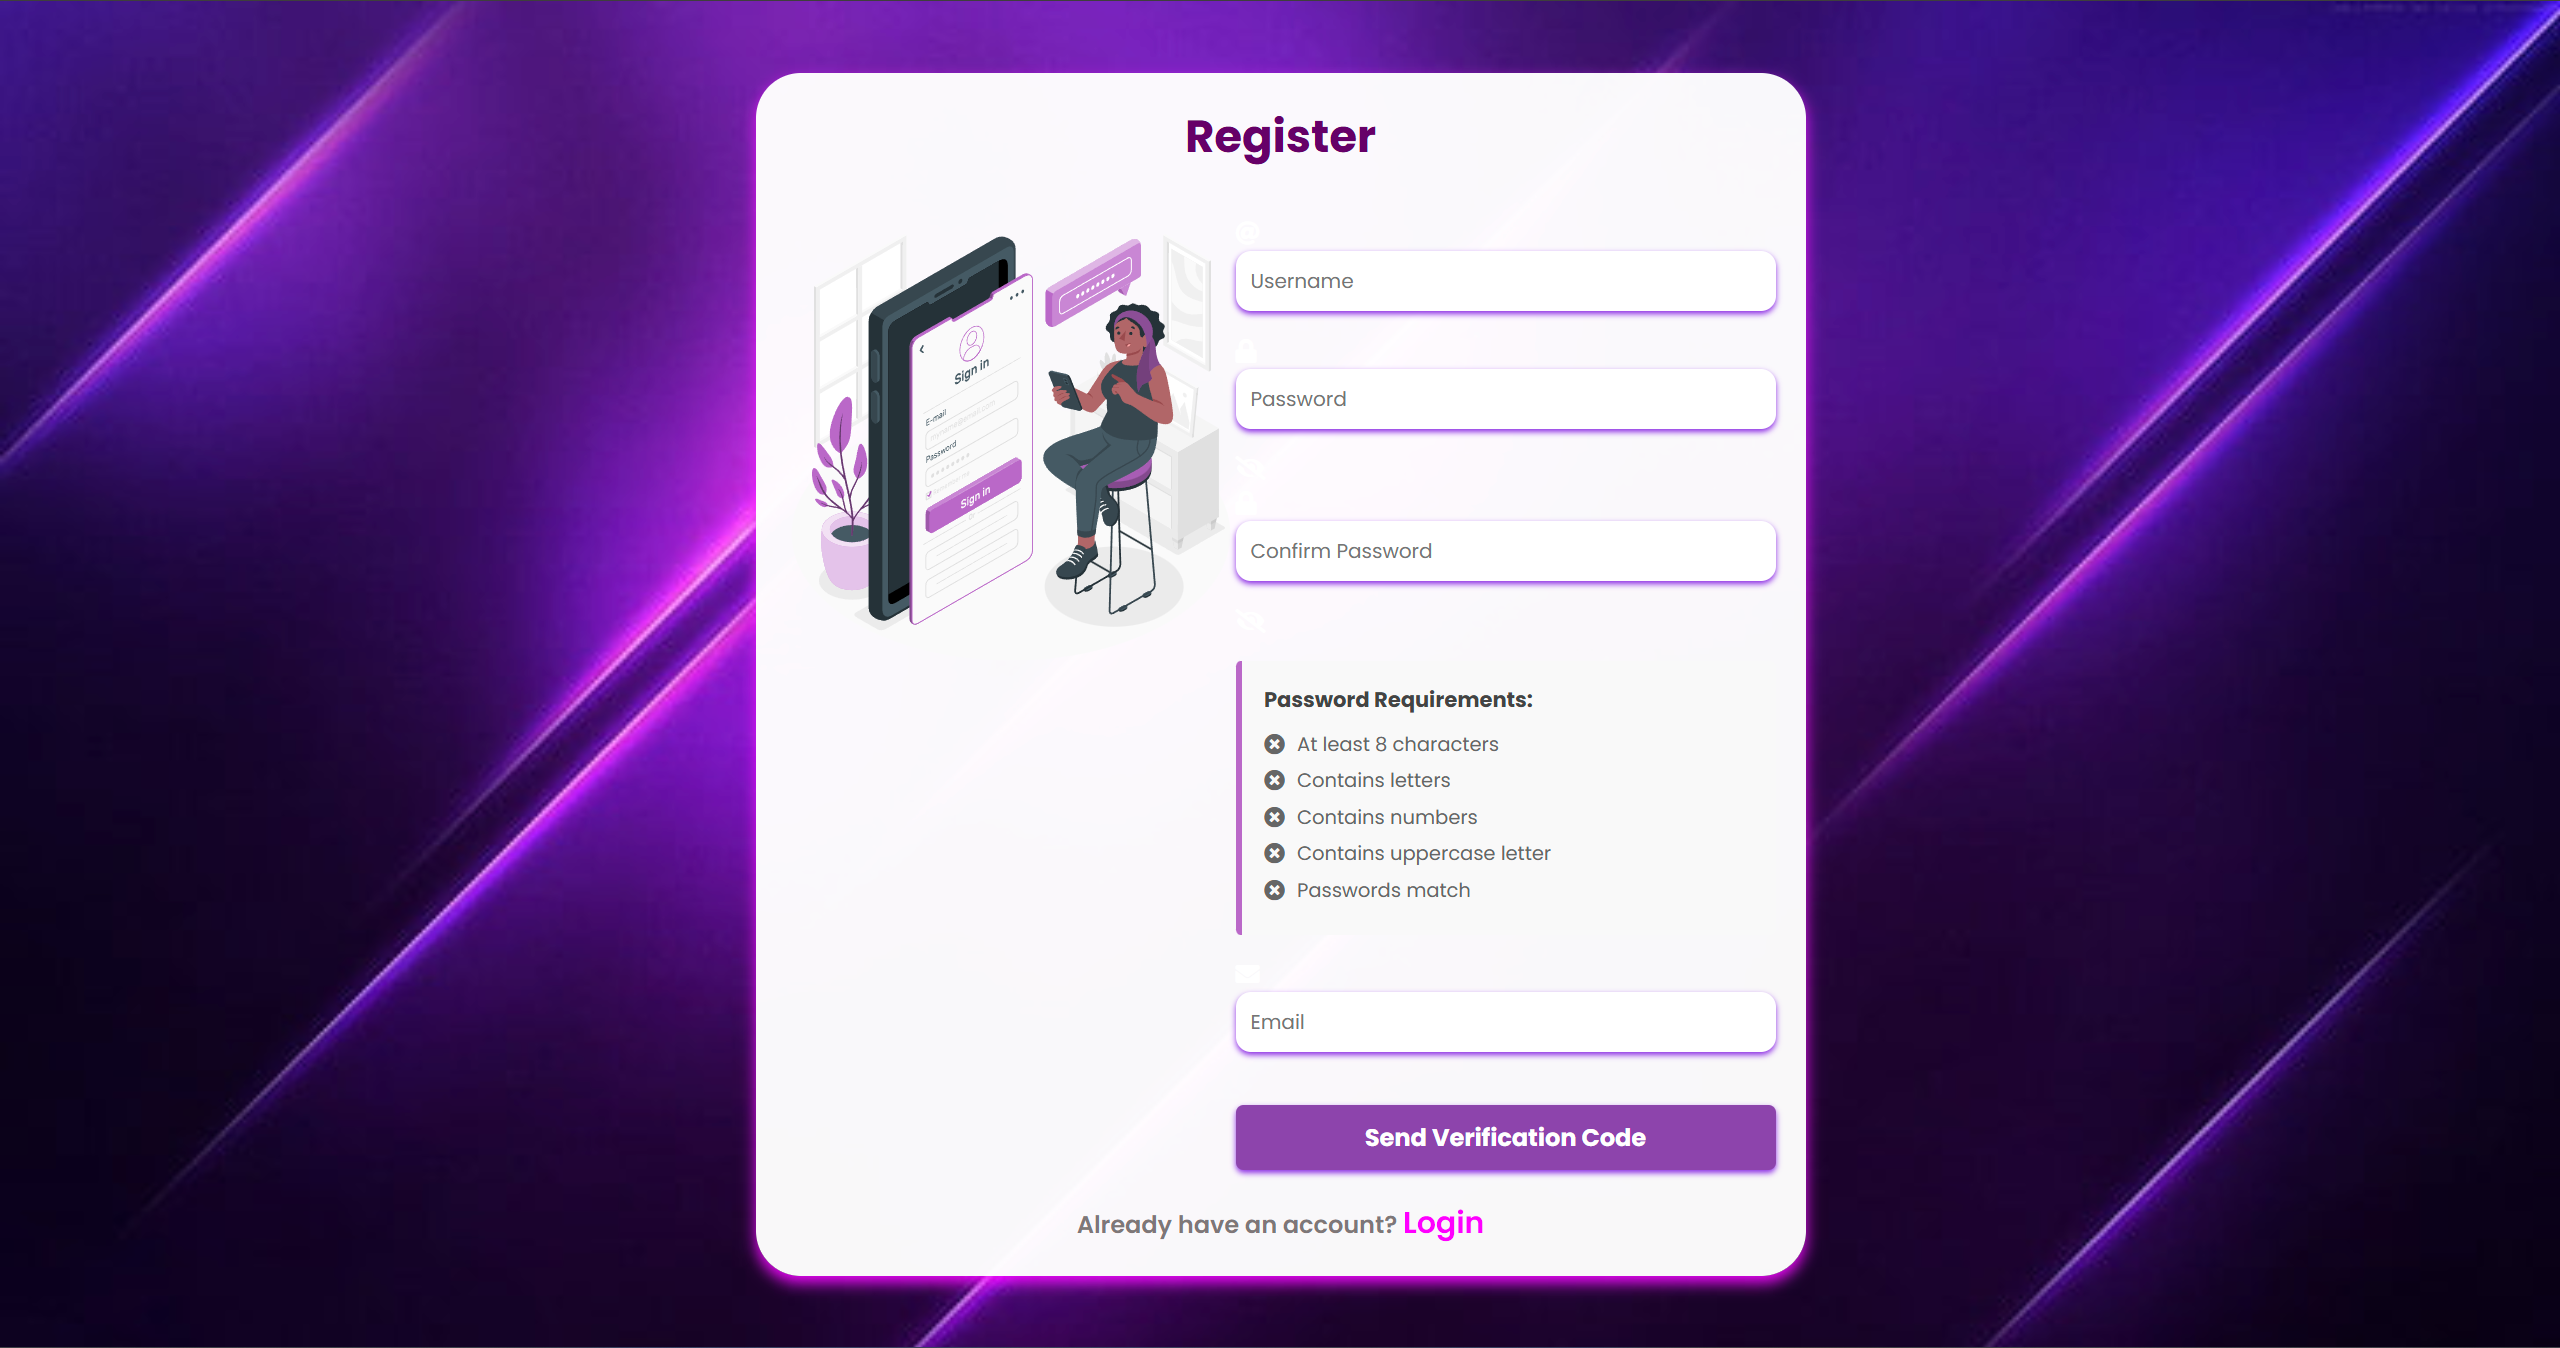
\includegraphics[width=0.5\textwidth]{images/registration_screenshot.png}
    \caption{Registration interface of the system}
    \label{fig:registration}
\end{figure}
After registration, a database message is generated in MongoDB containing all the user's personal data, including email address, password, etc. After logining, the user is redirected to the system's AI dialogue interface, where the same dialogue messages are machine-learned, classified and stored in the appropriate database.

There are several critical assets in the system and these are protected in the following to maintain privacy, data integrity and secure operation. The details are analysed below:

\begin{enumerate}
    \item user login and registration information: This information can be exposed when accessing web pages, submitting web pages, and in the MongoDB database, so if not stored in MongoDB using the bcrypt hash algorithm, successful intrusion by outsiders could lead to impersonation or unauthorized access.
    \item MongoDB databas: Data protection in the database is the most important part, which includes all legitimate personal data entered into the system. It also stores user conversations, including private data and illegal queries, which must be classified and monitored to avoid contamination of the local database.
    \item Session identifiers: This type of data is stored in client cookies across a Flask session and, if intercepted, a malicious user can access user data without logging in.
    \item System configuratio: System configuration information is unlikely to be exposed, but it is a risk. The env file stores the key and connection string; once exposed, visitors can read the database data directly, compromising the encryption and security of the database.
    \item HTTP communication channels: HTTP traffic is very easy to capture with Wireshark. Therefore, the use of HTTPS is also part of effective data management and security.
\end{enumerate}

\subsection{Threat model}
Systems without built-in defences are exposed to a number of threats, all of which can have a serious impact on our websites and users, including privacy breaches and loss of profit. 

Cyberattacks are the most common, immediate and obvious threat. Considering that users' names, emails, account names and passwords are directly or indirectly used and stored in our system, it is the most important task to prevent this information from being collected and exploited by attackers. 

Insider threats are another key risk category. Since data is stored in MongoDB, developers and administrators with direct access to the database may accidentally or maliciously access or even leak user information. 

Emerging risks, though less immediate, should be proactively considered in system design. Further research into encryption algorithms for long-term data is needed due to the ongoing development of quantum computing technology, which may lead to the obsolescence of today's encryption algorithms in the future.

\subsection{Assess impact and prioritize threats}
The most direct method of attack in cyberattacks is to brute-force a website's user login information and attempt to log in. In the absence of defensive measures, the attacker can use automated scripts to systematically guess user credentials, especially for users who use weak passwords and repeated passwords, the success rate of this attack is very high. 

Furthermore, because we use MongoDB as the data storage tool in our system, we are vulnerable to NoSQL injection threats. If user input is embedded directly into the query object without rigorous cleaning or architectural enforcement, an attacker may be able to manipulate authentication logic or extract sensitive data. Unlike traditional SQL injection, NoSQL injection in document-based databases is typically less well known and therefore more easily overlooked by developers. 

Nevertheless, the system is vulnerable to distributed denial-of-service (DDoS) attacks, especially via HTTP flooding. While a high volume of requests for login or registration endpoints does not compromise user information and privacy, it can exhaust server resources and cause legitimate users to temporarily lose access to the service. 

Insider threats are inherently impactful due to the privileged nature of access although it is less common. In the absence of auditing or fine-grained access control, a single point of abuse can lead to a massive privacy breach.

Quantum computing presents a serious challenge to modern cryptographic assumptions. Many widely used encryption schemes, including RSA and elliptic curve ciphers (ECC), are theoretically vulnerable to quantum attacks, most notably through the Shor algorithm. Once quantum computers reach a sufficient number of quantum bits (\$n\$) and error-correction capabilities, these cryptosystems are no longer reliable.

We used the STRIDE threat classification model to classify and evaluate the threats identified in the system, specifically assessing the nature and severity of each threat to determine its priority:

\begin{itemize}
    \item T1 - Plain Text Transfer (I: Information Leakage)
    
    The project initially transmitted credentials via HTTP, which poses a serious risk according to the STRIDE model. As previously mentioned, it is very easy to perform packet sniffing (e.g. Wireshark) on the same network, which would compromise the privacy of all user input.
    
    \item T2 - SQL Injection (S: Spoofing and E: Privilege Escalation)
    
    SQL injection attempts allow an attacker to impersonate a valid user and this method will be very effective when the database is not encrypted. Although this can be partially mitigated using bcrypt password checking, it still allows unauthorised access to user sessions. Therefore, this remains a high priority.
    
    \item T3 - Forced login (D: Denial of Service)
    
    Although a forced login scenario or DDOS network attack cannot significantly steal or decrypt databases and private customer information, it can also cause some disruption to the client or server and degrade performance. Therefore, they have medium to high priority.
    
    \item T4 - Session hijacking (S: Spoofing)
    
    If an attacker gets hold of a valid session cookie, they can bypass authentication. Although the impact is high, the likelihood is low.
    
    \item T5 - $.env$ file leak (I + E)
    
    Leaking $.env$ files can lead to information disclosure and privilege escalation, especially if $MONGO\_URI$ or $AES\_KEY$ is compromised. However, depending on the misconfiguration, this is less likely to happen in a controlled deployment.
    
\end{itemize}


\subsection{Data Sources and attacks set-up}
\subsubsection{Wireshark's HTTP message capture}
We start with the registration information as an example as shown below. After registering the user information and clicking submit, we use Wireshark to add the filtered information header as shown in Figure X to the same network segment, which will show the record of all the requests submitted under that segment. 
So after clicking on that record we can get the relevant user information in Figure \ref{fig:Demo Registration}.

\begin{figure}[htb]
    \centering
    \begin{minipage}{0.5\textwidth}
        \centering
        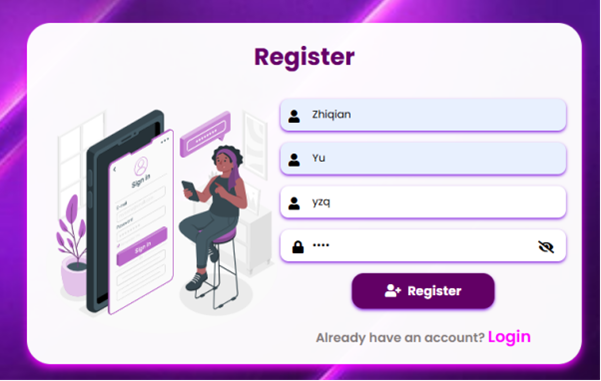
\includegraphics[width=\textwidth]{images/Demo Registration.png}
        \caption*{(a) Demo Registration}
    \end{minipage}
    \hfill
    \begin{minipage}{0.5\textwidth}
        \centering
        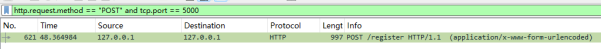
\includegraphics[width=\textwidth]{images/Capture Information.png}
        \caption*{(b) Capture Information}
    \end{minipage}
    \hfill
    \begin{minipage}{0.5\textwidth}
        \centering
        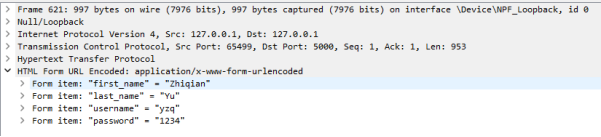
\includegraphics[width=\textwidth]{images/Information content.png}
        \caption*{(c) Information content}
    \end{minipage}
    \hfill
    \begin{minipage}{0.5\textwidth}
        \centering
        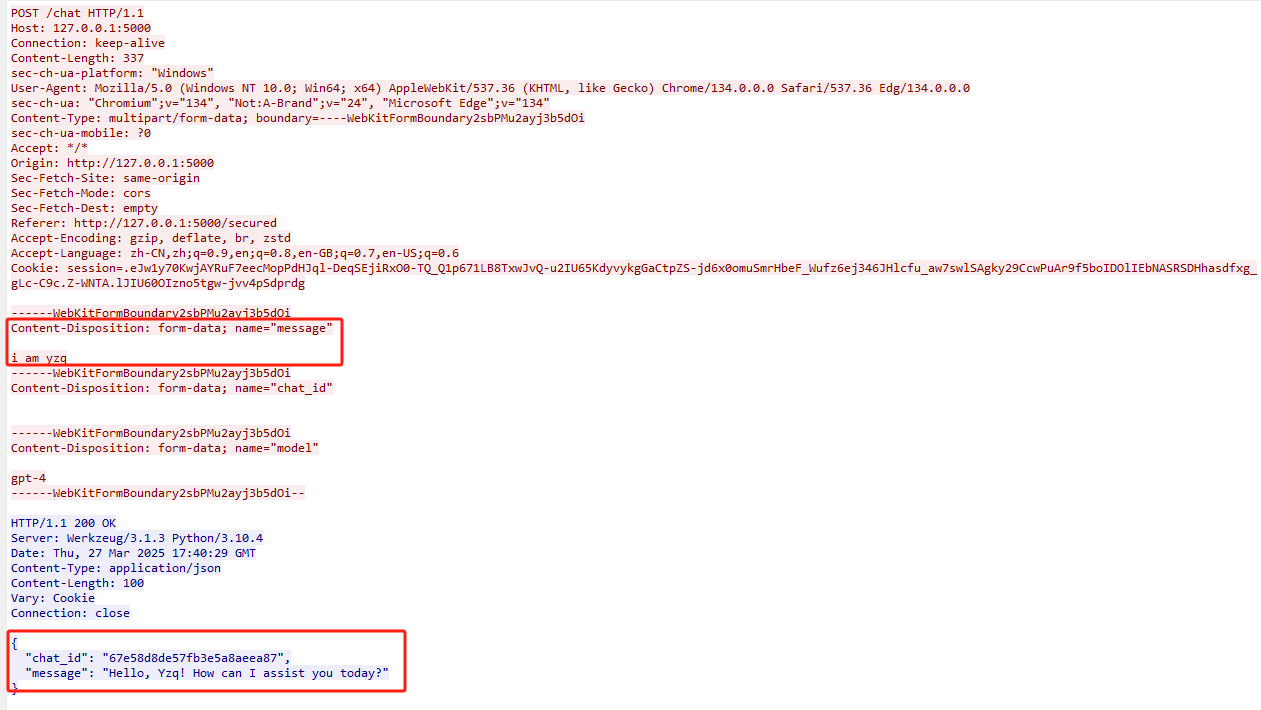
\includegraphics[width=\textwidth]{images/AI dialogue Information content.png}
        \caption*{(d) AI dialogue Information content}
    \end{minipage}
    
    \caption{Wireshark's HTTP message capture}
    \label{fig:Demo Registration}
\end{figure}

\subsubsection{Session Hijacking}
After the user has successfully logged in, there is a legitimate session cookie in the browser, at this point we can use Wireshark to get the value of this cookie through a packet grabber, inject the cookie into our own browser, and then visit the /secured page. This will allow us to access the /secured page without logging in, thus obtaining the user's privacy directly. 
As shown in Fig. \ref{fig:cookie}, we have captured a login request in wireshark that contains a cookie message.

\begin{figure}[htb]
    \centering
    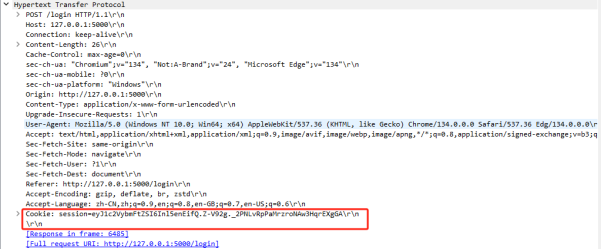
\includegraphics[width=0.5\textwidth]{images/Information of Cookie.png}
    \caption{Information of Cookie}
    \label{fig:cookie}
\end{figure}

After getting this cookie information, open the login screen and enter the information shown in Fig. \ref{} in the Console, we will see that the system has recognised the content of the cookie. 
So we enter the page we need to go to in the web port which is http://127.0.0.1:5000/secured and we can see that we have successfully jumped to the user interface.

\begin{figure}[htb]
    \begin{minipage}{0.5\textwidth}
        \centering
        \includegraphics[width=\textwidth]{images/}
        \caption*{(a) Session Hijacking}
    \end{minipage}
    \hfill
    \begin{minipage}
        \centering
        \includegraphics[width=\textwidth]{images/}
        \caption*{(b) Session Hijacking}
    \end{minipage}
    
    \caption{Information of Cookie}
    \label{fig:cookie}
\end{figure}






\section{Coursework 2: Security \& Privacy Defense Strategy (up to 5 pages)}
\subsection{Security (or Privacy or both) Interaction/visualisation/actuation system}
\subsection{Threats inferences and insights}
\subsection{Regulation and Ethical considerations}
\subsection{Scalability, Innovation \& Enterprise Considerations}

\vfill\pagebreak

% References should be produced using the bibtex program from suitable
% BiBTeX files (here: strings, refs, manuals). The IEEEbib.bst bibliography
% style file from IEEE produces unsorted bibliography list.
% -------------------------------------------------------------------------
\bibliographystyle{IEEEbib}
% \bibliography{refs}

\end{document}
